\documentclass[twocolumn]{article}
\usepackage[top=1.1in, left=0.85in, right=0.85in]{geometry}

\usepackage{url}
\usepackage{code}
% \usepackage{cite}
\usepackage{amsmath}
\usepackage{amssymb}
\usepackage{graphicx}

\pagestyle{empty}

\usepackage{ulem}
% go back to italics for emphasis, though
\normalem

\usepackage{natbib}

\newcommand\comment[1]{}
\newcommand\sfrac[2]{\!{}\,^{#1}\!/{}\!_{#2}}

\begin{document} 

\title{New results in $\sfrac{k}{n}$ Power-Hours}
\author{Dr.~Tom~Murphy~VII~Ph.D.\thanks{
Copyright \copyright\ 2014 the Regents of the Wikiplia
Foundation. Appears in SIGBOVIK 2014 with the chagrin of the
Association for Computational Heresy; {\em IEEEEEE!} press,
Verlag-Verlag volume no.~0x40-2A.
\yen 0.00}
}

\renewcommand\th{\ensuremath{{}^{\textrm{th}}}}
\newcommand\st{\ensuremath{{}^{\textrm{st}}}}
\newcommand\rd{\ensuremath{{}^{\textrm{rd}}}}
\newcommand\nd{\ensuremath{{}^{\textrm{nd}}}}
\newcommand\at{\ensuremath{\scriptstyle @}}

\renewcommand\>{$>$}
\newcommand\<{$<$}
\newcommand\kn{\ensuremath{\sfrac{k}{n}\,}}
\newcommand\bmsl{BM$s$L}

\newcommand\any{\ensuremath{\textrm{?}}}
\newcommand\nocup{\text{\sout{\ensuremath{\cup}}}}
\newcommand\fullcup{\ensuremath{\uplus}}
\newcommand\emptycup{\ensuremath{\cup}}
\newcommand\overcup{\ensuremath{\cap}}
\newcommand\scup[1]{\ensuremath{\cup\!\!\!{}^{{}_{#1}}}}

\newcommand\nodrink{\ensuremath{\Rightarrow}}
\newcommand\drink{\ensuremath{\stackrel{{}^{\textrm{+}}}{\Rightarrow}}}
\newcommand\qdrink{\ensuremath{\stackrel{{}^{\textrm{?}}}{\Rightarrow}}}

\date{1 April 2014}

\maketitle \thispagestyle{empty}

\begin{abstract}
We correct for inebriated missteps, using computational methods to
establish new bounds in generalized \kn Power-Hour theory.
\end{abstract}

\vspace{1em}
{\noindent \small {\bf Keywords}:
  generalized binge drinking, maths,
  finite-state automata,
  abstract interpretation
}

\section*{Introduction}
A 2012 paper by Blum, Martens, Murphy, and Lovas\cite{algorithms}
introduced the \kn Power-Hour, a fractional variant on the well-known
drinking game. In a traditional Power-Hour, participants drink one
shot of beer per minute for 60 minutes. Since 5--6 beers in an hour
sometimes have adverse effects, some players opt for an attenuated
version of the game wherein fewer than 60 shots are consumed. However,
since the game is frantic and played simultaneous with others, it is
critical to have a mechanical procedure for performing the attenuated
Hour. The framework by Blum {\em et al.}, hereafter BMML, gives a
handful of simple operations that can be used to define a state
machine among $p$ players:
\begin{itemize}
  \item At the beginning of each minute, each player has at most one
    shot glass in front of him or her
  \item The shot glass must be in one of three states: Filled \fullcup,
    empty \emptycup, or overturned \overcup
  \item Atomically, each player performs an action based only on the
    state of his or her cup. If not in possession of a cup (written
    \nocup), the only action is to do nothing. With a cup:
  \begin{itemize}
    \item The player may drink \drink, or not drink \nodrink
    \item The player may pass the cup in any state to any player (a
      fixed player per action)
    \item However: If the cup is filled and the player did not drink,
      it must be passed in the filled state
    \item A player may not receive more than one cup in the same round
  \end{itemize}
\end{itemize}

Every assignment of rules and starting condition to $p$ players yields
a deterministic outcome, though some of these are illegal (because
they result in two or more cups being passed to the same player in
some round). For legal games, the outcome is that the $p$ players have
consumed $k_i$ shots of beer where $1 \leq i \leq p$ and $0 \leq k_i
\leq 60$. For the traditional power hour, the player starts with an
empty cup, at each step drinks,\!\footnote{In practice, this is done
  by filling the cup and then drinking it.} leaves the cup empty, and
passes to herself.

While the authors made a mostly clear definition of BMML and presented
some initial results, these results contained multiple serious errors
and the paper abruptly switches notation and assumptions several
times, and rambles incoherently. By their own admission, the authors
were drinking while they wrote it, taking only one hour to do so.
Don't drink and derive, kids!

This paper revisits the problem of BMML from a modern, sober
perspective, clarifies some of the original results, and presents
several new ones and a few conjectures. It is based on several pieces
of software, whose source is available online.\!\footnote{ \url{http://sourceforge.net/p/tom7misc/svn/HEAD/tree/trunk/powerhour/} }

\section{One-player \kn Power-Hours}

The goal of the \kn Power-Hour is to attenuate the number of drinks
consumed by the $p$ players, and its expressive power comes from the
ability to encode some state in the orientation of the cups, and
propagate that state via passing them from player to player. Even
without passing cups, the ability for a single player to attenuate his
drinking is nontrivial. Playing drinking games alone is sad indeed,
but the solo \kn Power-Hour still has practical applications. When
playing a Power Hour with others, if each player's desired $k$ is
attainable through solo methods then there is no need for passing
cups, which simplifies the ergonomics considerably. A common case is
where some of the players would like to do half--Power-Hours, which is
easily achieved in BMML by transitioning \emptycup\ to \fullcup\ without
drinking and \fullcup\ to \emptycup\ by drinking, and passing to
oneself.\!\footnote{There are many variations, but this was the
  strategy used many times in practice before being generalized to
  BMML.}

A full list of attainable \kn Power-Hours where $p=1$ appears in
Figure~\ref{fig:solo}. Possible values of $k$ are $\{ 0, 1, 2, 20, 29,
30, 31, 40, 58, 59, 60 \}$. The BMML paper claimed that the possible
values were $\{0, 1, 2, 20, 30, 40, 58, 59, 60 \}$, describing 31 for
example as ``super impossible.'' Achieving 31 is somewhat interesting.
One way to do it is to start with \emptycup, and use the rule that
\emptycup\ means drink and then fill the cup. We then use the rule
that \fullcup\ means drink and flip the cup, and \overcup\ means don't
drink and fill the cup. Essentially we use \emptycup\ to mean ``this
is the very first state'' and then take shots on alternating minutes
by using \overcup\ and \fullcup\ to encode the parity. Exploiting
non-steady-states like this (Figure~\ref{fig:solo31}) is how we
achieve $k$ that does not share many factors with $n$.

\begin{figure}[ht]
\begin{center}
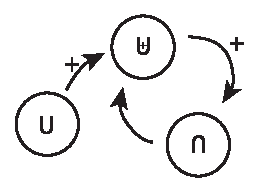
\includegraphics[width=0.90 \linewidth]{solo31.pdf}
\end{center}\vspace{-0.1in}
\caption{State machine that achieves $k=31$ in a solo BMML Power Hour.
  $+$ on an edge means the player drinks. The disembodied incoming
  edge is the start state. The player always passes to herself.}
\label{fig:solo31}
\end{figure}

It is tractable to work out the possibilities for the solo case by
hand, though apparently not while drinking~\cite{algorithms}. These
results were generated by a computer program, which is probably
necessary for $p>1$. In the remainder of the paper, I'll describe
several different approaches for exploring this space, and
generalizations of it, computationally.

\begin{figure}[ht]
\begin{center}
\begin{tabular}{c|ll}
$k$ & start & rules \\
\hline
0  &   \nocup    &  \emptycup \nodrink \any     , \overcup \nodrink \any      , \fullcup \nodrink \any \\
1  &   \emptycup &  \emptycup \drink \overcup   , \overcup \nodrink \overcup  , \fullcup \nodrink \any \\
2  &   \emptycup &  \emptycup \drink \fullcup   , \overcup \nodrink \overcup  , \fullcup \drink \overcup \\
20 &   \emptycup &  \emptycup \nodrink \overcup , \overcup \nodrink \fullcup  , \fullcup \drink \emptycup \\
29 &   \emptycup &  \emptycup \nodrink \overcup , \overcup \nodrink \fullcup  , \fullcup \drink \overcup \\
30 &   \emptycup &  \emptycup \drink \overcup   , \overcup \nodrink \emptycup , \fullcup \nodrink \any \\
31 &   \emptycup &  \emptycup \drink \fullcup   , \overcup \nodrink \fullcup  , \fullcup \drink \overcup \\
40 &   \emptycup &  \emptycup \drink \overcup   , \overcup \nodrink \fullcup  , \fullcup \drink \emptycup \\
58 &   \emptycup &  \emptycup \nodrink \overcup , \overcup \nodrink \fullcup  , \fullcup \drink \fullcup \\
59 &   \emptycup &  \emptycup \nodrink \overcup , \overcup \drink \overcup    , \fullcup \nodrink \any \\
60 &   \emptycup &  \emptycup \drink \emptycup  , \overcup \nodrink \any      , \fullcup \nodrink \any \\
\end{tabular}
\end{center}
\label{fig:solo}
\caption{All the possible $k$ for a solo Power-Hour in BMML. A
  superscript $+$ means that the player drinks. The symbol \any\ means
  that any cup state can be used in that position. Note that 29 and 58
  require wasting a shot of beer (the game ends with the shotglass
  full); all the others but 31 permit a variant where a shot is wasted
  as well. We do not concern ourselves much in this report with these
  leftover shots.}
\end{figure}

\section{Two-player \kn Power-Hours}

For more players, the number of possible configurations explodes.
Let's make the following definitions to bound the size:
\begin{itemize}
\item $t = 4$, the number of starting states (\fullcup, \emptycup,
  \overcup, \nocup)
\item $a = 2 \times p \times 3$, the number of actions given a cup.
  The player can drink or not drink, pass to any player, and in 3
  configurations (\fullcup, \emptycup, \overcup)
\end{itemize}
Then the number of configurations is bounded by $(t \times a^3)^p$. For
$p=1$ this was just 864. For $p=2$ it is 47,775,744; for $p=3$ it's
12,694,994,583,552, already beyond the limits of straight enumeration.

\comment{
fun ct (p : IntInf.int) =
  let val s = 4
      fun pow n 0 = 1
        | pow n m = n * pow n (m - 1)
      val a = 2 * p * 3
   in
      pow (s * pow a 3) p
  end
}

However, this is just an upper bound. For one thing, the base of the
exponent is actually bounded by
$$
  t \times a^2 \times a_{\textrm{filled}}
$$
where
$a_{\textrm{filled}} = (p \times 3) + p$ (the actions that can be taken on
\fullcup, where if the player does not drink, then he must pass the
cup \fullcup).

\comment{
fun ctb (p : IntInf.int) =
  let val s = 4
      fun pow n 0 = 1
        | pow n m = n * pow n (m - 1)
      val af = p * 3 + p
      val a = 2 * p * 3
   in
      pow (s * pow a 2 * af) p
  end
}

The values for $p \in \{1,2,3\}$ are still 576; 21,233,664;
3,761,479,876,608. There are a few other simplifications possible.
Many of these games are illegal because they result in multiple cups
being passed to the same player in some turn. These are difficult to
exclude analytically, but there are some sufficient conditions; for
example, if two players pass to the same player no matter their input
state, and every player starts with a cup, then their cups always
collide. There are also many games that are isomorphic. For one thing,
\emptycup\ and \overcup\ are not distinguished in the rules at all, so
any two configurations where these are simply swapped has the exact
same outcome. Likewise for permuting the players.

21 million configurations is no big deal for a modern computer. A
simple SML program computes all of the configurations and runs them;
ones that are found to be illegal are rejected. (It implements the
first simplification having to do with \fullcup\ when generating the
configurations, since it can be done statically.) All of the possible
outcomes are shown as black squares in Figure~\ref{fig:powerhour2player}.

\begin{figure}[ht]
\begin{center}
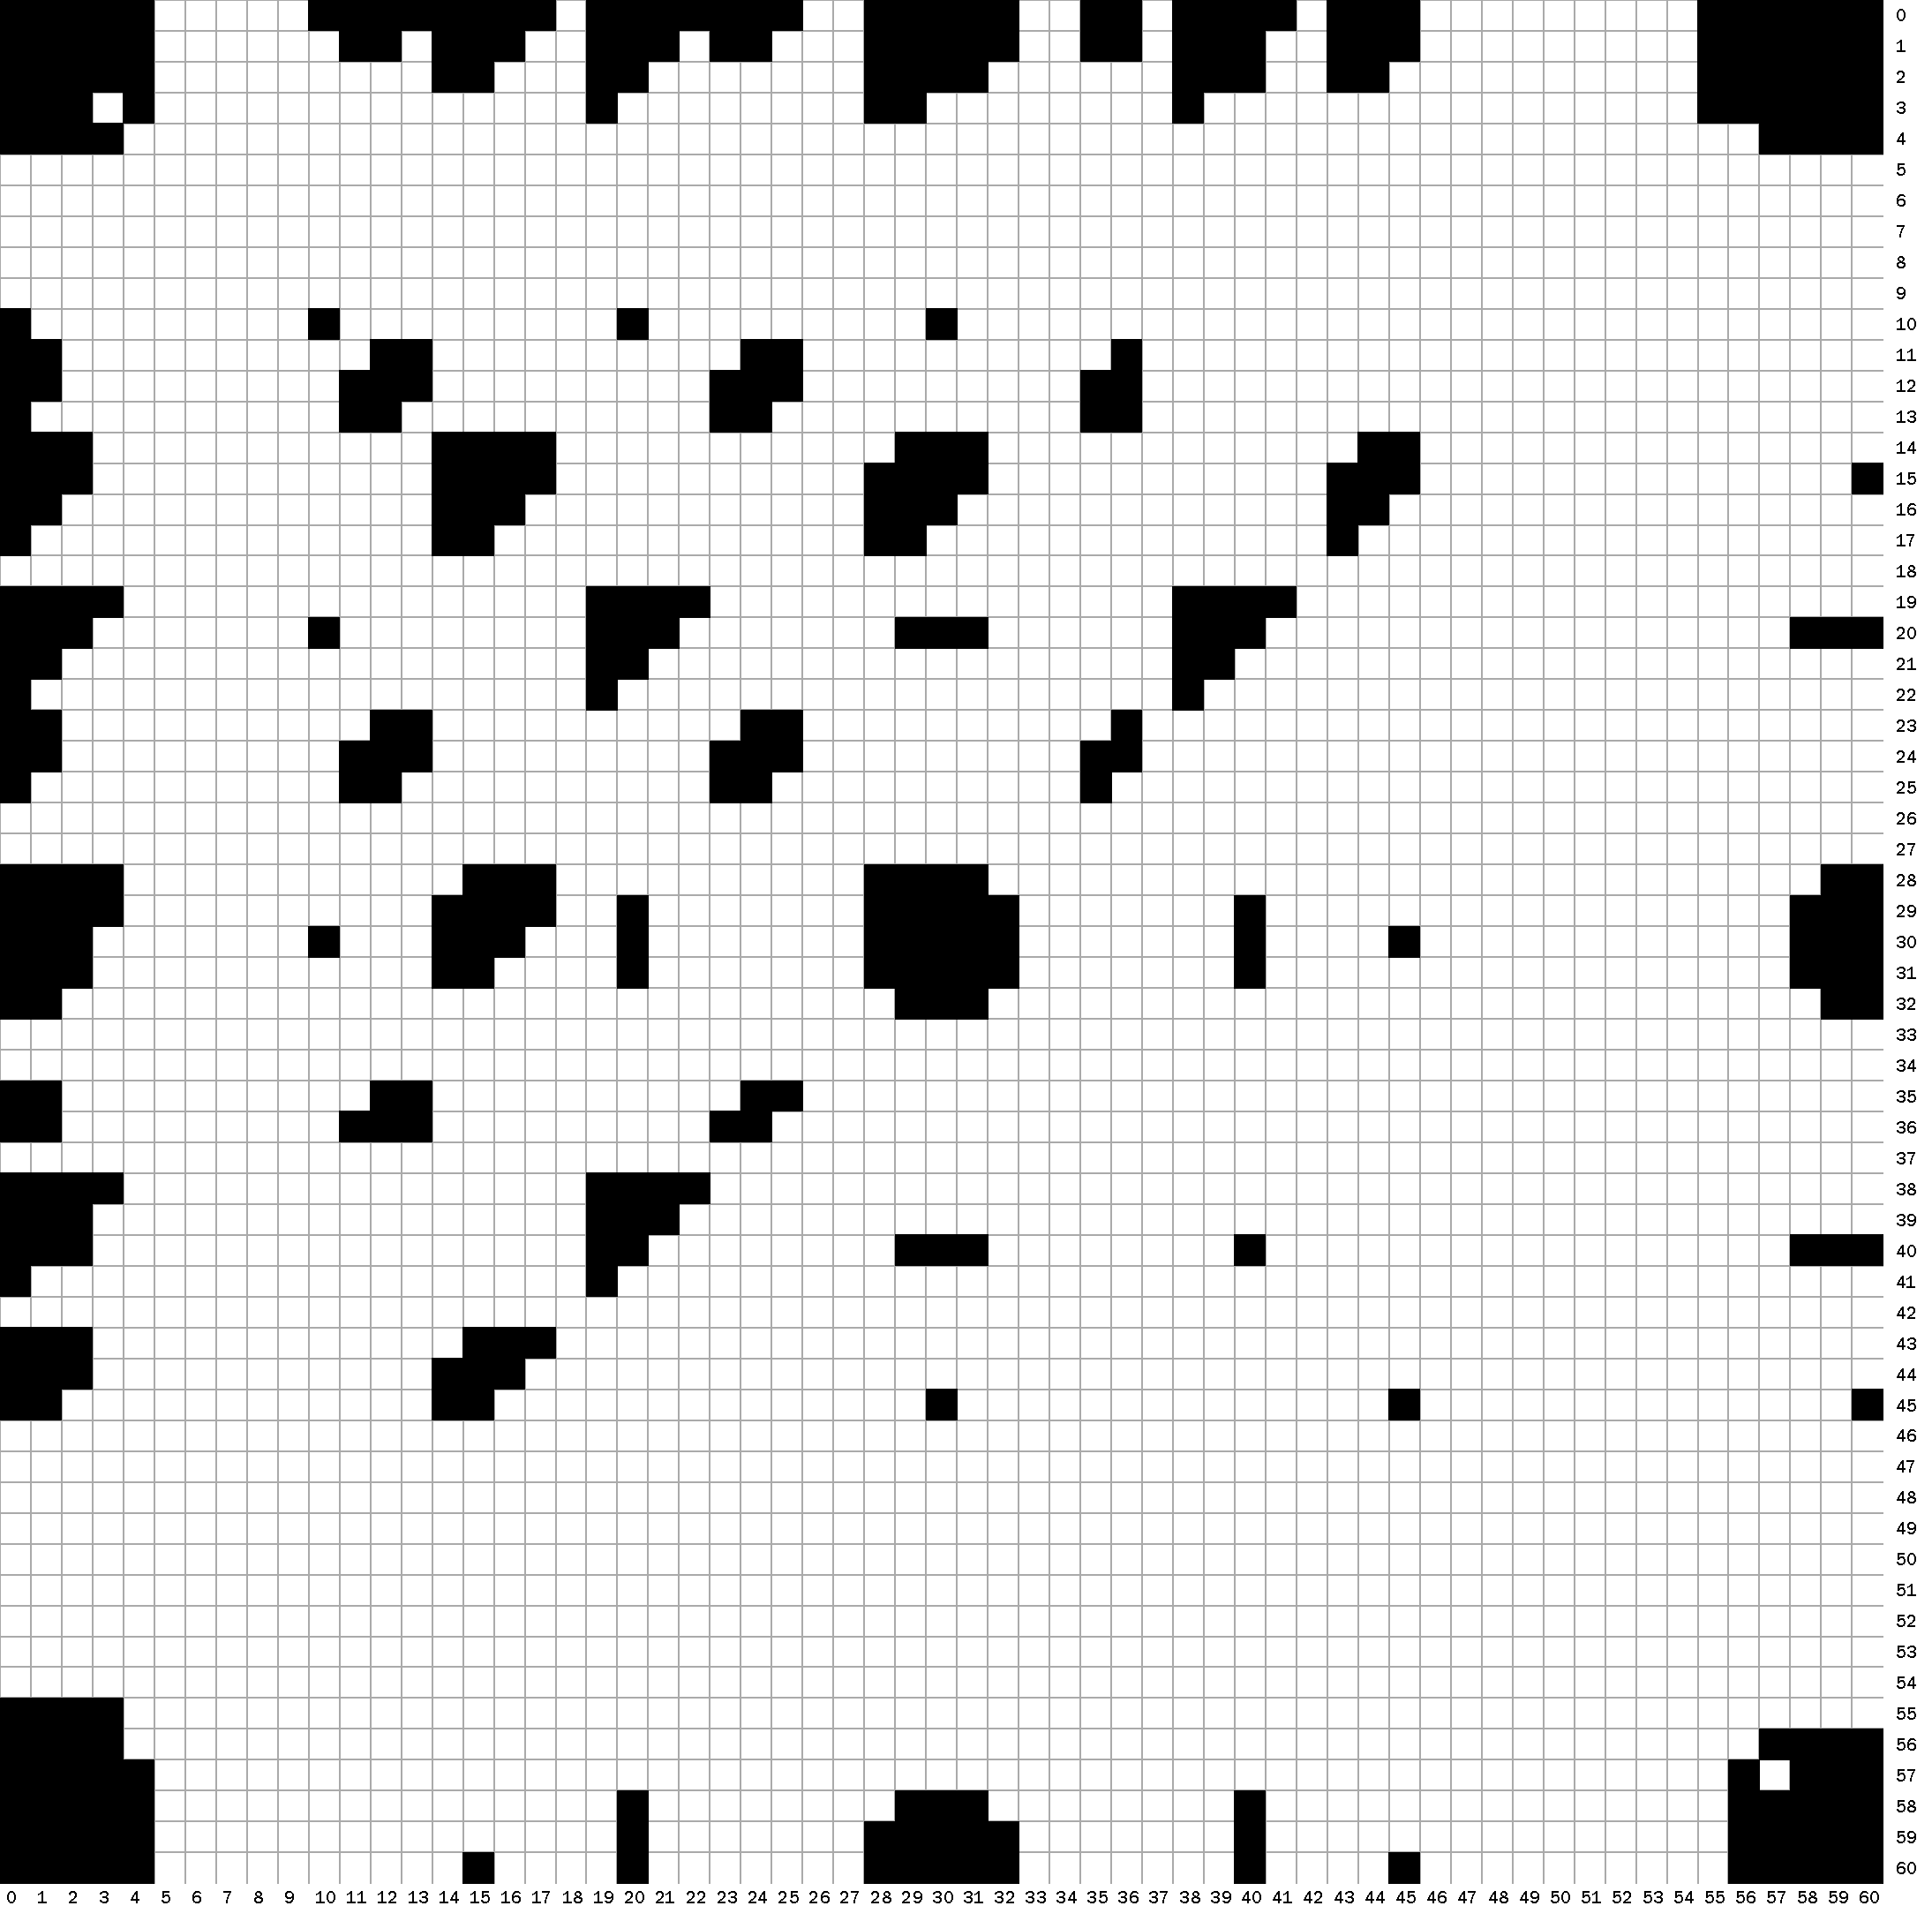
\includegraphics[width=0.90 \linewidth]{powerhour2player.pdf}
\end{center}\vspace{-0.1in}
\caption{All of the possible outcomes ($k$) for the two players in a
  BMML Power-Hour. The matrix is symmetric, of course, since the players
  are interchangeable.}
\label{fig:powerhour2player}
\end{figure}

Each cell represents a pair of $\langle k_1, k_2 \rangle$ for the
number of shots imbibed by players 1 and 2. 454 of the $61^2 = 3721$
combinations are achievable. Note that column 0 represents the case
where player 1 drinks nothing. It dominates the matrix in the sense
that if $\langle k_1, k_2 \rangle$ is achievable, then $\langle 0, k_2
\rangle$ is as well. Most of the time it is easy to see how this is
done: Take the configuration that produces $\langle k_1, k_2 \rangle$
and do the same, but player 1 simply performs her actions without
drinking. This works except for the case where player 1 receives a
\fullcup\ and passes it in a state other than \fullcup. The player
can't simply not drink, as this is illegal (the beer must be emptied,
and BMML does not permit such messy reductions). It is curious that
this does not affect the result; I discuss this further in
Section~\ref{sec:conjectures}. Another interesting column is the last
one, which represents outcomes of the form $\langle 60, k_2 \rangle$,
where the first player achieves a full Power-Hour. This of course
includes all of the $k_2$ achievable solo (the players can just do
their thing without interacting). But some new $k$ are now achievable:
$\{ 3, 4, 15, 28, 32, 45, 56, 57 \}$. Interacting with a player doing
a full Power-Hour still affords us a few additional bits of
information that can be used to attenuate the other player's
consumption. The solution for $45$ is instructive, and appears in
Figure~\ref{fig:dual45}.

This is a useful result, but it may be the case that someone wants to
drink exactly 27 shots of beer, which is not possible with just two
players in BMML. There are two avenues to explore: Adding more 
players, and generalizing BMML. We begin with the three-player case.

\begin{figure}[ht]
\begin{center}
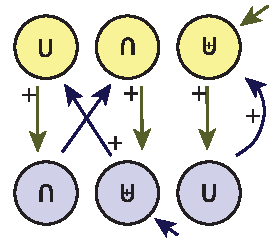
\includegraphics[width=0.90 \linewidth]{dual45.pdf}
\end{center}\vspace{-0.1in}
\caption{State machine that achieves $\langle k_1=45, k_2=60 \rangle$
  in a two-player BMML Power Hour. The bottom row of states are for
  player 1, who drinks 45, and the top for player 2, who drinks 60.
  Clearly, player 2 must drink at every step. The players always pass
  to each other, with the two cups exchanging hands each turn. The
  cycles for the two cups are disconnected; one alternates between
  \fullcup\ in player 2's hand and \emptycup\ in player 1's (cycle
  of length 2), drinking on each turn. This cycle yields 30 drinks
  for each player. The other cycle is of length 4; player 2 drinks
  on every step (as we know), and player 1 every 4\th\ step, yielding
  15 more drinks for a total of 45.
% [60,45] wasting 2: 12 game(s) like 
% [(start F, U=>D*@1 D=>F*@1 F=>U*@1),
%  (start F, U=>F*@0 D=>D@0 F=>U*@0)]
}
\label{fig:dual45}
\end{figure}

\section{Three-player \kn Power-Hours}

With 3.7 trillion possible configurations, enumeration is not
feasible. But as we observed before, many of these combinations are
illegal (they result in a player recieving two cups), and many are
isomorphic to one another. By being clever about how we explore the
configurations, testing ``all'' the three-player configurations
becomes feasible.

Here is a one-player BMML configuration that illustrates a particular
kind of redundancy:
\vspace{1em}
\begin{tabular}{cc}
start \emptycup & \emptycup \drink \emptycup 
 \quad \fullcup \drink \overcup
 \quad \overcup \nodrink \fullcup
\end{tabular}

The cup starts empty, and at each step the player fills it and drinks
(traditional Power-Hour). The player also has rules for the case that
she observes a full or overturned cup. {\em It does not matter what
  these are} because they can never be used. This example is trivial,
but there are many ways that the execution of a configuration can be
indifferent to some of its content. Another is a two player
configuration like
\vspace{1em}
\begin{tabular}{rcccc}
player 1 & start \emptycup & \emptycup \drink \overcup \at 1
 & \fullcup \drink \overcup \at 2
 & \overcup \nodrink \fullcup \at 1 \\
player 2 & start \emptycup & \emptycup \nodrink \emptycup \at 1
 & \fullcup \drink \overcup \at 1
 & \overcup \drink \fullcup \at 2 \\
\end{tabular}
where the $\at n$ notation means to pass the cup in that state to
player $n$. In this case, the first thing the players do is to
pass both of their cups to player 1, which is illegal and ends the
game. Again, none of the other rules are ever used.

In order to explore what is possible in three-player games, we exploit
this redundancy with a technique like abstract
interpretation~\cite{abstract}. The start state is always used, so we
begin by enumerating all assignments of start states to players. There
are only $4^p$. Every other rule starts out undetermined, maybe written
like this:

\begin{tabular}{cc}
start \emptycup & \emptycup \qdrink \any
 \quad \fullcup \qdrink \any
 \quad \overcup \qdrink \any
\end{tabular}

Now we execute programs as before, and hope that we never encounter a
situation where we depend on a rule. If we finish without ever using
one of the \any\ rules, we evaluated a potentially large group of
configurations all at once. During the execution of a configuration,
if we need to use a rule that is currently marked \any, we explore all
of the possibilities for that spot. This is accomplished by a loop
that looks like the following (in Pseudo SML):

\begin{code}
val queue = (* all abstract configurations *)
val results = (* map from (k_1, k_2) 
                 to example *)
\codeskip
fun loop nil = (* done *)
  | loop (h :: t) =
      let
        val res = evaluate h
      in
        insert (results, res);
        loop t
      end handle Expand l => loop (l @ t)
\codeskip
fun evaluate config =
   (* ... *) 
   case rulefor cup of 
      QuestionMark =>
         raise Expand expandedconfigs
    | (* ... *)
\codeskip
val () = loop queue
\end{code}

The key trick here for keeping the code under control is to
iteratively evaluate the configurations as usual, but if we find a
\any, then we abort the current simulation with an exception that
carries along the set of configurations that expand the current one in
just that position. This wastes some work (and we often need to
restart multiple times per abstract configuration), but not much: If a
rule is used at all, it is usually used in one of the first few
rounds.

With this technique, we can simulate all possible two-player games
with just 15,744,259 game-minutes simulated (with naive enumeration it
would be 1.2 billion) in less than 2 seconds on a crappy old computer.

% XXX TODO: Display in 3D cube.
It is also feasible overnight to enumerate all three-player games. The
results are three-dimensional, of course, but we can display the
outcomes for two of the players in the familiar presentation
(Figure~\ref{fig:3and2}). Note that $\langle k_1, k_2, k_3 \rangle$ is
achievable for any $k_1 \in \{ 0 \ldots 60 \}$, $k_2 \in \{ 0, 1, 2 \}$,
and some unknown $k_3$ (projected out of this display). This is a
significant improvement over what was achievable in BMML with two
players. It suggests that with enough friends willing to follow a
program, some set of people are likely to be able to achieve any
amount of drinks between them (if they have the ability to construct
the right rule set!); see Section~\ref{sec:conjectures}.

The sheer number of configurations for 4 or more players makes these
exact enumeration techniques infeasible. However, we have other
avenues for generalization (and exploration), which are investigated
in the next chapter.

% Total steps 15744259. Took 1982 ms
% Total steps 15744259. Took 2080 ms

% #100000 queue 31 min 16 6059166 states/sec 100000 config/sec
% #200000 queue 20 min 16 8762059 states/sec 200000 config/sec
% #300000 queue 35 min 16 12125162 states/sec 300000 config/sec
% #400000 queue 25 min 16 7613270 states/sec 200000 config/sec
% Total steps 15744259. Took 2101 ms

% There are 16 games before splitting.
% #100000 queue 31 min 16 6059166 states/sec 100000 config/sec
% #200000 queue 20 min 16 8762059 states/sec 200000 config/sec
% #300000 queue 35 min 16 6062581 states/sec 150000 config/sec
% #400000 queue 25 min 16 7613270 states/sec 200000 config/sec
% Wrote 454 possibilities to possible-2.txt
% Total steps 15744259. Took 2162 ms

% Wrote 454 possibilities to possible-2.txt
% Total steps 895743. Took 292 ms

% Wrote 2787 possibilities to possible-5cup-60min-2player.txt
% Total steps 6890640495. Took 8161324 ms

% on metroid
% Wrote 37560 possibilities to possible-3.txt
% Total steps 1393736865. Took 1,545,217 ms

\begin{figure}
\begin{center}
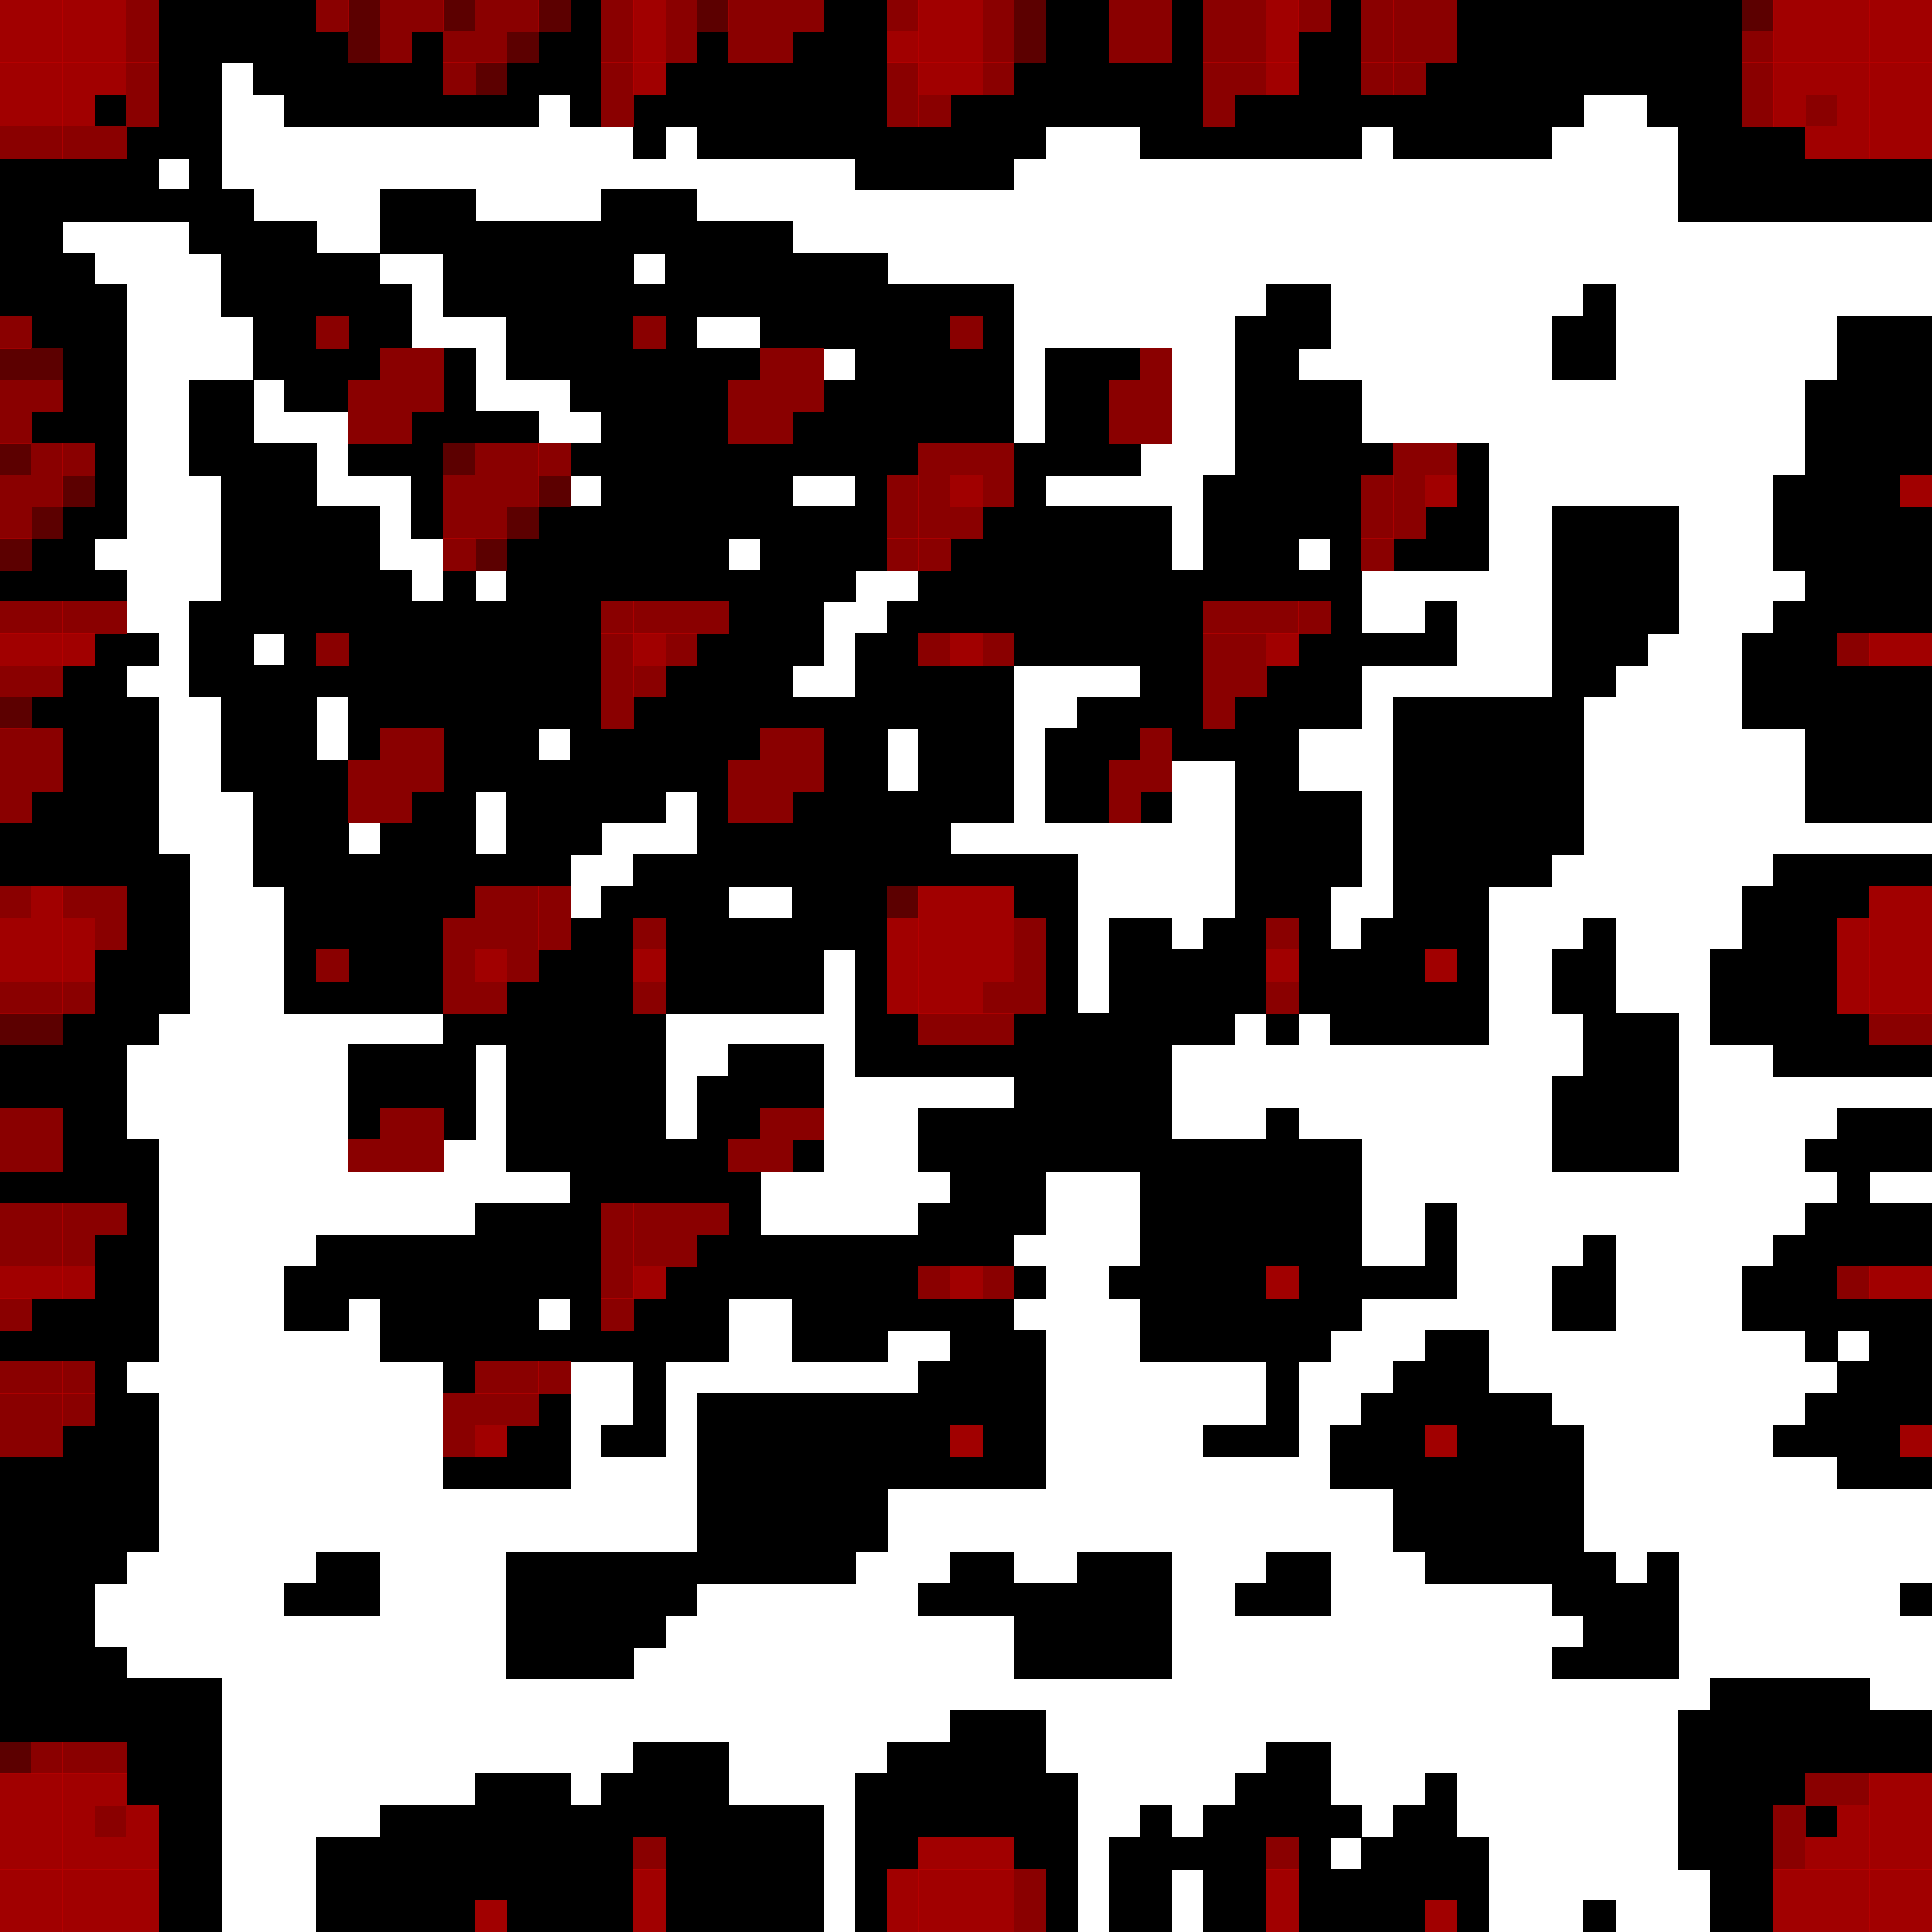
\includegraphics[width=0.90 \linewidth]{3and2.pdf}
\end{center}\vspace{-0.1in}
\caption{Outcomes possible for the first two players in all different
  3-player power hours (black), overlayed by all possible outcomes
  outcomes for 2-player power hours (red). Mainly included because
  it looks pretty sweet. The outcomes that are possible with three
  players are a superset of those with two, which is intuitive: We
  can add a third player to any game who just does nothing.}
\label{fig:3and2}
\end{figure}

\section{Generalized BMML}

Like any drinking game, there are several arbitrary things about BMML.
While we will not tamper with its essence (for example, allowing beer
to be spilled from a cup without drinking it), there are some other
variables to adjust. The most naturally flexible is the number of cup
states. We will always have \fullcup, a cup with beer in it. In BMML
we also have \emptycup\ and \overcup. But why not $\supset$ (cup
turned on its side, facing west) or $\stackrel{\wedge}{\cup}$ (an
upright cup with a cocktail umbrella on it)?

We define \bmsl, where $s$ is the number of distinct cup states. By
convention, the 0\th\ cup state will be the filled cup \fullcup\ since
it has special rules. The remainder will be \scup{i} for $i \in \{ 1,
\ldots, s - 1 \}$. BMML is BM3L where we've just renamed \emptycup\ to
\scup{1}, and \overcup\ to \scup{2}.

Clearly, more cups give us more expressive power, and should allow us
to reach more outcomes. To illustrate, recall the construction of
$k=31$ in the solo BM3L game (Figure~\ref{fig:solo31}). It has a
length-2 cycle alternating between two cup states, where the player
drinks on every other turn. The third state is just used once as a
drinking lead-in to make the total 31 rather than 30. With an
additional cup state, we can straightforwardly transform this into a
game with an outcome of $k=32$ by extending the prelude with another
state where the player drinks. Of course, the expressive power is not
just limited to such extensions; we now can create cycles of new
lengths, admit the possibility of more disconnected cycles, and so on.

It is easy to enumerate the 1-player \bmsl\ games. These appear in
Figure~\ref{fig:soloncups}. The interesting range for $s$ is $\{ 1
\ldots 8 \}$.\!\footnote{It's not clear that BM0L should be considered
  legal as the rules speak of a 0\th\ cup, but it is degenerate
  anyway.} At 8 cup states, the player can achieve any amount in a
solo game. Importantly, this extends to any number of players in BM8L,
because the players can pass to themselves and not even interact.

\begin{figure}
\begin{center}
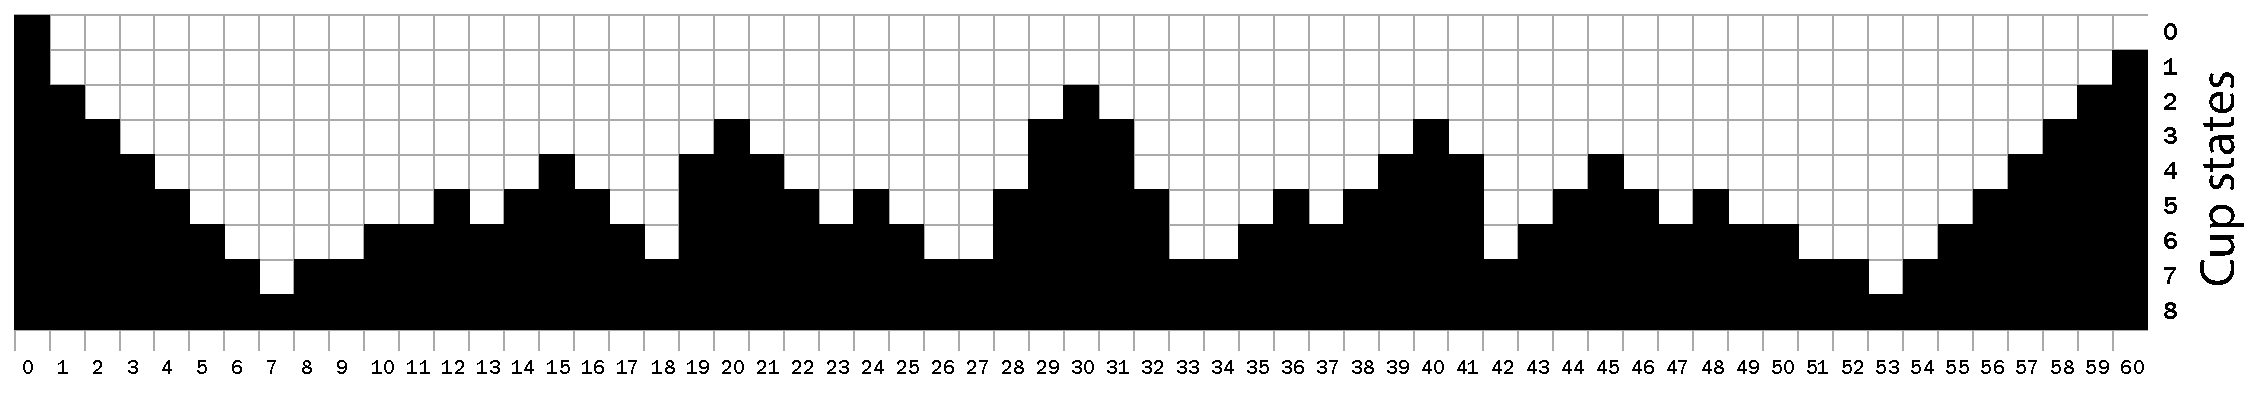
\includegraphics[width=\linewidth]{soloncups.pdf}
\end{center}\vspace{-0.1in}
\caption{Possible outcomes for \bmsl\ with a single player. The
  vertical axis shows an increasing number of cup states, and the
  horizontal axis shows the achievable values of $k$ drinks. With no
  cup states, it is only possible to drink nothing. By convention, the
  0\th\ cup is the special ``filled'' state, so it is only possible to
  drink on every turn (60) or never (0). As we add more cup states,
  the number of achievable states strictly increases; with 8 cup
  states we can drink any amount. 7 and 53 drinks are the most
  elusive, and can only be done with 8 cup states.}
\label{fig:soloncups}
\end{figure}

The two-player case is much more interesting. We've already enumerated
all the possible outcomes for BM3L
(Figure~\ref{fig:powerhour2player}). It is computationally tractable
to enumerate them for $s < 6$. The set of achievable outcomes in
BM$s$L is always contained within BM$(s+1)$L, because we can embed a
game from the former into the latter by just never producing the
additional cup state and having any arbitrary rule for it. Therefore,
we show these results in a composite grid where more and more states
are reachable as we increase $s$ (Figure~\ref{fig:composite2player}).

\begin{figure}
\begin{center}
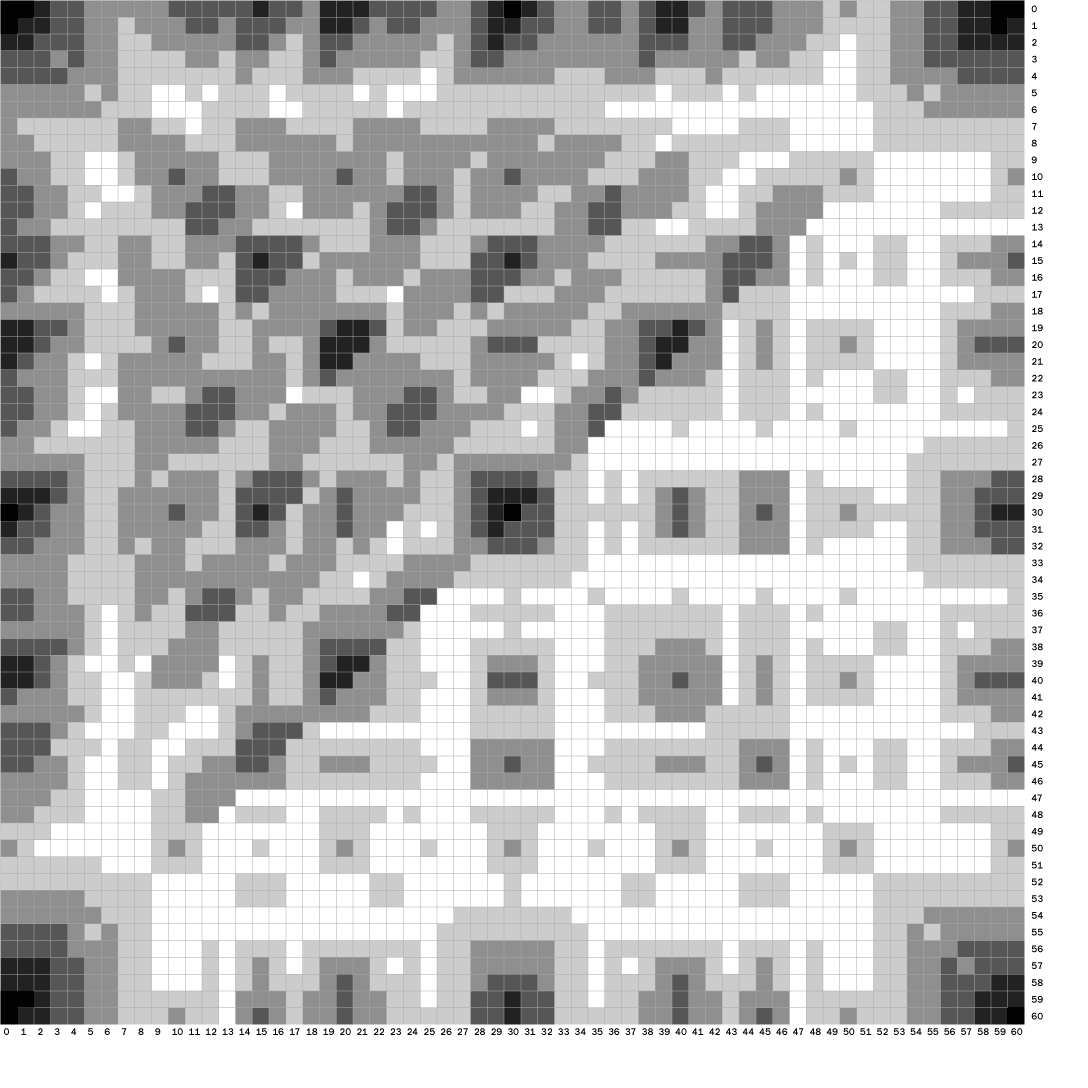
\includegraphics[width=0.90 \linewidth]{composite2playermock.png}
\end{center}\vspace{-0.1in}
\caption{What's achievable for two players in a generalized \bmsl\ game,
  with $s$ ranging from 1 cup state (darkest) to 5 (lightest).
% 6 cupstates ran overnight and got here:
% #26186200000 queue 109 min 49 466729 states/sec 796272 config/sec
}
\label{fig:composite2player}
\end{figure}

In order to efficiently enumerate BM5L, I improved the algorithm
again. Observe that the ``drink'' action associated with a rule
usually does not affect anything but the final outcome. The only
exception is that in the rule for \fullcup, the player must drink if
passing in a state other than \fullcup. Putting this aside for a
moment, note that we can just count the number of times each rule was
executed for each player, producing an $s$-dimensional vector $[ d_1,
  \ldots, d_s ]$ for each player. That player is able to achieve many
different drink totals, specifically, $d_1 \times r_1 + \ldots + d_s
\times r_s$ where $r_i$ is 1 if the player should drink on that rule
and 0 if not. Simulating a game this way is even more like abstract
interpretation (we leave a concrete value free and compute a formula
rather than an integer), and allows us to evaluate many concrete games
at once. At the end, we simply plug in every legal value for $r_i$ for
each player and insert those games into the database. This last step
is where we must tend to the exception around \fullcup. We may not set
$r_0$ to 0 if the player ever passes \fullcup\ in a non-full state. A
very close approximation would be to insist that $r_0 = 1$ if the rule
in the \fullcup\ position does not output as \fullcup, but this is
inexact, as that rule may never be executed.\!\footnote{We may be able to
  argue that in that case, there always exists another game that does
  not violate this condition. But I think it is simpler to just
  implement the rules.} Instead, during simulation we keep track of
whether each player ever actually passed a non-full cup from the
\fullcup\ state. If so, then we force $r_0 = 1$, which attends to this
special case. \label{sec:linear}

Although this makes earlier enumerations extremely fast and BM5L
quite quick, 2-player BM6L ran 26 billion concrete states overnight
and made only modest progress. In the absence of fancier techniques
for reducing the state space, we must resort to different, inexact
approaches.

\section{Sampling games}

To establish a result like ``BM5L cannot achieve $\langle 47, 27
\rangle$'' we really need to enumerate all the BM5L games. (Or make
some ad hoc proof of the fact, which seems quite difficult.) However,
to prove an existence result like ``BM7L can achieve $\langle 33, 49
\rangle$'' we only need to have a single example configuration that
produces that result. Therefore, we may be able to improve our bounds
on what is possible (or generate conjectures) by sampling random
configurations.

Sampling is actually much easier than enumeration. There is no need to
leave rules abstract. It is also easy to stop and restart because
there is no state other than the matrix of what we've found. I use the
SML {\tt textformat} library~\cite{textformat} to serialize and
deserialize the matrix (which then makes it easy to generate these
graphics in a separate program). There are a handful of interesting
aspects:

\paragraph{Generating a random configuration.} To generate a random
game, we can just fill in all of the slots (destination and cup state
for each rule, starting cup state) uniformly at random. Many of these
will be illegal, but they fail very quickly at runtime; a lazy and
pragmatic way to ``filter'' to legal game. It is not simply a matter
of generating all the permutations on $p \times s$ nodes, by the way.
Multiple cups can pass through the same player on cycles of different
periods, as long as they do not collide within the 60 steps, and
acyclic preludes (Figure~\ref{fig:solo31}) are important and useful.
For a uniformly random 2-player BM7L configuration, 29.23\% (measured
empirically) are legal. However, we will see later that we do not want
to spend so much time exploring configurations where one or both
players start without a cup; these are very limited. Therefore, the
configuration generator is biased towards producing a cup in the
starting states most of the time.

\paragraph{Symmetry.} We can get more bang for the buck by considering
some obvious symmetries. When a simulation finishes and we have an
outcome $\langle k_1, \ldots, k_p \rangle$, it is clear that any
permutation of $k_1 \ldots k_p$ is also achievable. We insert every
permutation of the drink counts into the database, along with the
permuted example configuration. Better still would be to only store
the outcomes in some normalized form (e.g. require that $k_1 \leq
\ldots \leq k_p$).

We already have exact results for two players in BM5L, so the next
uncharted territory is BM6L. The result after apparent convergence
appears in Figure~\ref{fig:samplebm6l}. The sampling procedure runs
for many hours before plateauing overnight with 95.65\% of the matrix
filled. This suggests that BM6L is not universal for two players, or
else the configurations for the missing cells are extremely
rare.\!\footnote{This is definitely a possibility, as new cells were
still appearing after exploring tens of billions of samples. However,
the gap here seems quite large.}

This approach scales much better than enumeration and is efficient for
all sorts of generalizations (it works best when the dimensionality is
low---i.e., two players---and the expressiveness is high---i.e., many
cup states). Since we already know BM8L is universal, the remaining
open problem is BM7L, whose results are in
Figure~\ref{fig:samplebm7l}. Indeed, after more than 30 billion
samples the matrix is completely filled in; we have found an example
configuration that achieves every outcome. Some of these were
extremely rare, such as the solution for $\langle 11, 53 \rangle$
(Figure~\ref{fig:dual11-53}). In BM7L, two players can drink any
amount.

\begin{figure}
\begin{center}
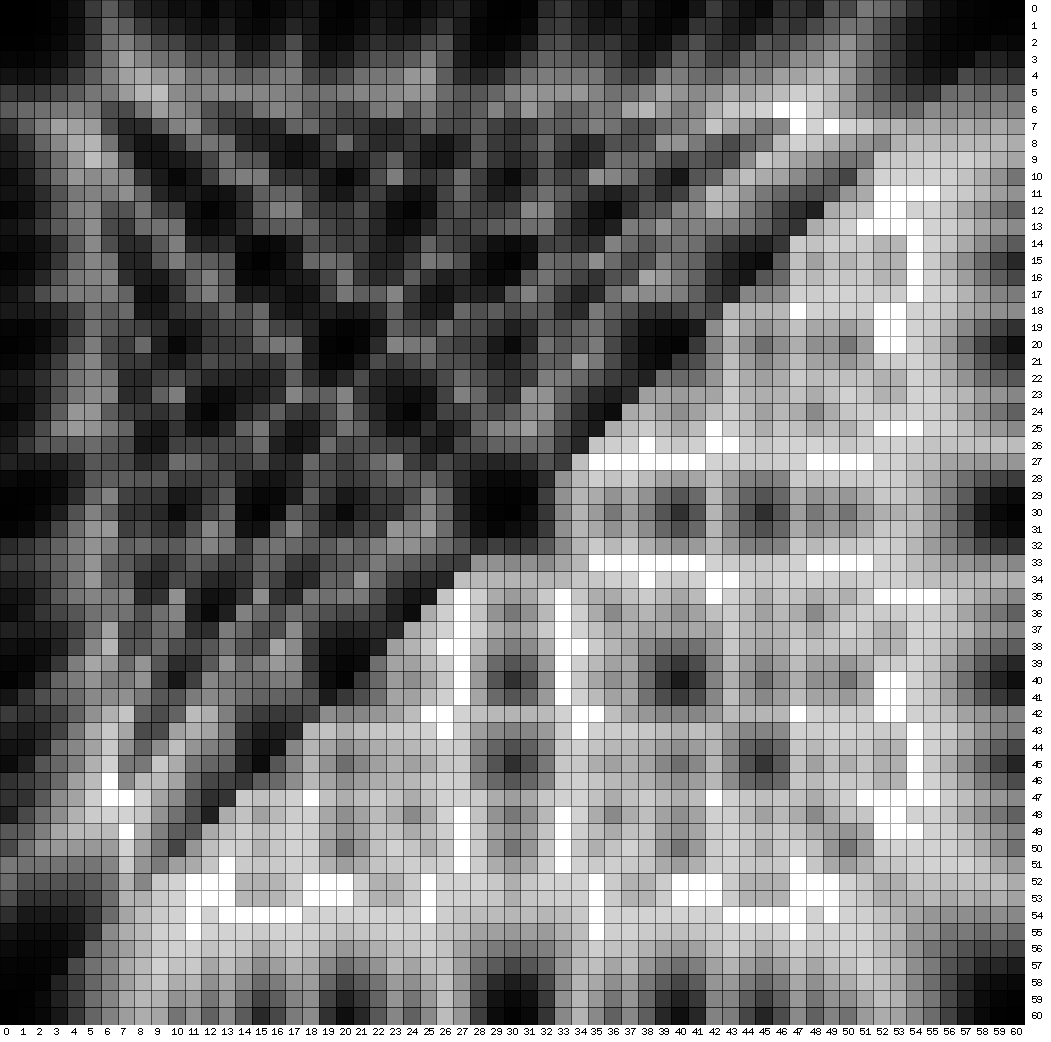
\includegraphics[width=0.90 \linewidth]{sample60min2players6states.png}
\end{center}\vspace{-0.1in}
\caption{ 37.1 billion samples of legal two-player BM6L
  configurations. Darker cells represent outcomes that occur more
  often; cells that are pure white never occurred and are likely to be
  unattainable. Note that the intensity represents the rank of
  occurrence, not the magnitude; in actuality, outcomes like $\langle
  0, 0 \rangle$ occur {\em much} more often than others.
  %
  95.65\% of the cells are filled.
}
\label{fig:samplebm6l}
\end{figure}

\begin{figure}[ht!]
\begin{center}
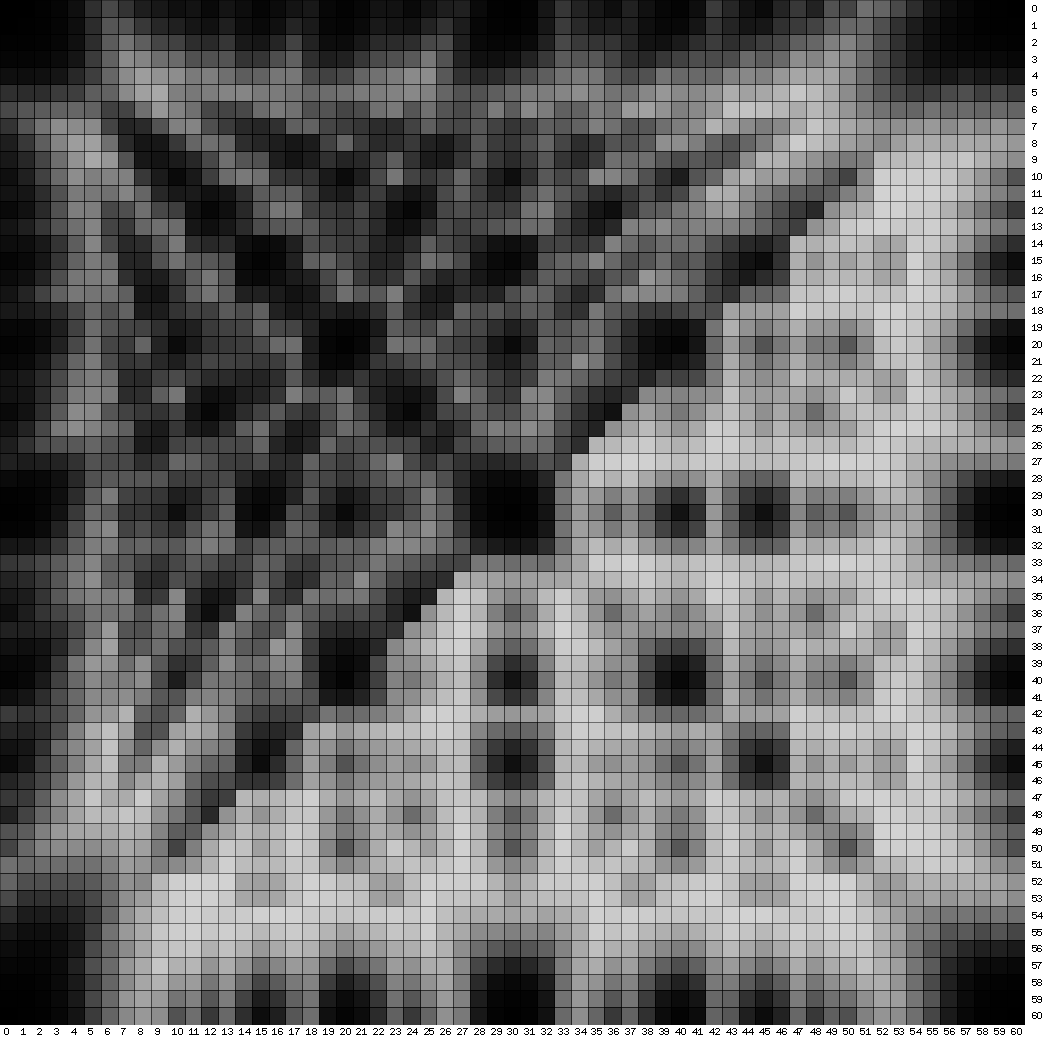
\includegraphics[width=0.90 \linewidth]{sample60min2players7states.png}
\end{center}\vspace{-0.1in}
\caption{ 30.7 billion samples of legal two-player BM7L
  configurations. Fewer configurations were sampled than in
  Figure~\ref{fig:samplebm6l} because they take somewhat longer than
  6-state games to simulate, and a smaller proportion of random games
  are legal. Moreover, we stop after finding a solution for every
  cell, proving that BM7L is complete! The last cells found---an
  earlier version of this paper held these as open problems!---were
  permutations of $\langle 11, 53 \rangle$
  (Figure~\ref{fig:dual11-53}) and $\langle 49, 53 \rangle$. Note that
  53 drinks was also unattainable in a solo BM7L power-hour; this may
  in some sense be the ``hardest'' number of shots to drink in \bmsl.
}
\label{fig:samplebm7l}
\end{figure}

\begin{figure}[ht!]
\begin{center}
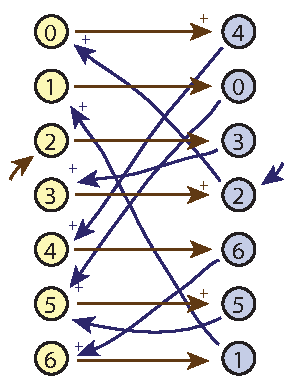
\includegraphics[width=0.90 \linewidth]{dual11-53.pdf}
\end{center}\vspace{-0.1in}
\caption{ A solution for the elusive $\langle 11, 53 \rangle$ two-player
  BM7L power hour! This one was found after 30.7 billion outcomes sampled,
  making it the most rare. By the end of the game, the two players are
  just passing back and forth two cups in state 5. A long lead-in beginning
  on the left-player's state 2 spans 12 different configurations (the 6
  cup states for the two players) before entering the length-two cycle.
  Both cups travel along this lead-in, with one three steps ahead of the
  other. The right player drinks on every step until reaching the cycle
  (and then never again) for 11; the left player drinks during the cycle
  plus a little extra during the lead-in for 53. This configuration is
  quite flexible because the two players can make fine adjustments to
  their drink total by drinking or not drinking on the lead-in rules,
  which are executed just once or twice.}
\label{fig:dual11-53}
\end{figure}


\section{The fractal geometry of \kn\ Power-Hours}

Note that all of the two-dimensional figures resemble one another even
though they are fundamentally different (adding players, adding
states, adding random trials). Even samples from BMML with three
players (3D projected to 2D), which is shown in Figure~\ref{fig:3d},
produces a similar pattern. This suggests that the combinatorial
problem (``what outcomes are reachable from finite state machines that
look kind of like this?'') has some geometric structure.

Some of the patterns are easy to explain. The top-left half of the
matrix is more populous than the bottom right, for example. This is
because we can bound the total number of drinks by $60 \times c$,
where $c$ is the number of cups active in the game (same as the number
of cups in the starting states). The top-left half is the region where
this sum is less than or equal to 60; in two player games, both
players must start with a cup in order to get an outcome in the
bottom-right half. We also see distinct clumps around 0, 15, 30, 45,
60; these correspond to simple fractions (``drink every other time'';
``drink three of four times'') of 60. This is intuitive because the
expressive power of BMML comes from the ability to form cycles of cup
states and drink on some fraction of them. Clumps are formed around
these values because of the possibility of preludes leading into the
cycles (Figures~\ref{fig:solo31}, \ref{fig:dual11-53}) that either
drink (adding to the total) or don't (subtracting from it). Minor
clumps form as echoes between the major ones, because a player may
participate in two cycles of different length
(Figure~\ref{fig:dual45}).

Of course, discretization effects compound and so the exact values of
cells are not neatly predictable. Moreover, clumps interfere by
overlapping; there are many different strategies for achieving
$\langle 33, 33 \rangle$. One way to make the basic structure more
visible is to extend the number of minutes that the game is played
for. Figure~\ref{fig:powerday3} shows the utterly unhealthy
three-player Power Day (BM3L). In it, the clumps become tiny dots,
but some relationship among them along lines is clear. Interior points
can probably be found as linear combinations of two of these lines;
we exploit that exact structure in Section~\ref{sec:linear}, in fact.

\begin{figure}
\begin{center}
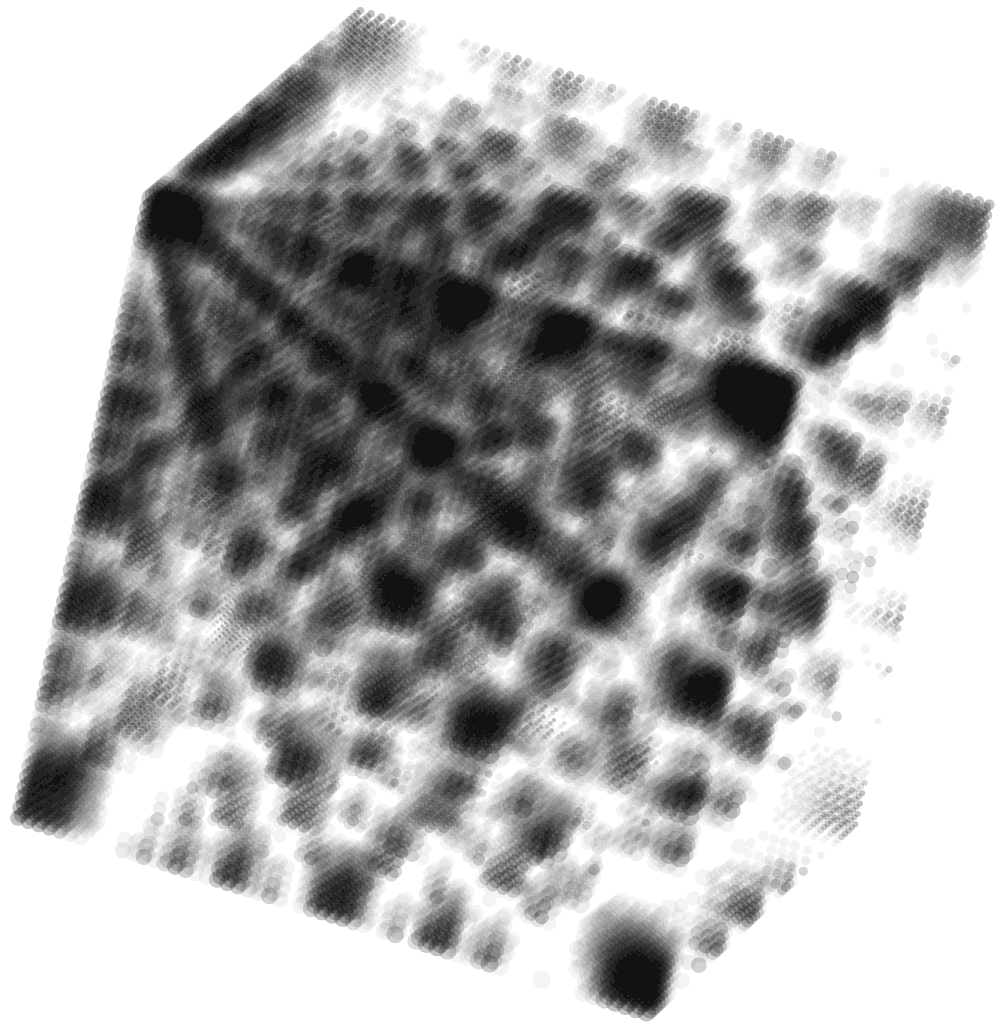
\includegraphics[width=0.90 \linewidth]{sample60min3players3states.png}
\end{center}\vspace{-0.1in}
\caption{490 million samples of three-player BMML Power Hours. The
  cube is rotated $15\,^{\circ}$ along each axis, the top-left corner is
  $\langle 0, 0, 0 \rangle$, and the bottom right is $\langle 60, 60,
  60 \rangle$. }
\label{fig:3d}
\end{figure}


\begin{figure}
\begin{center}
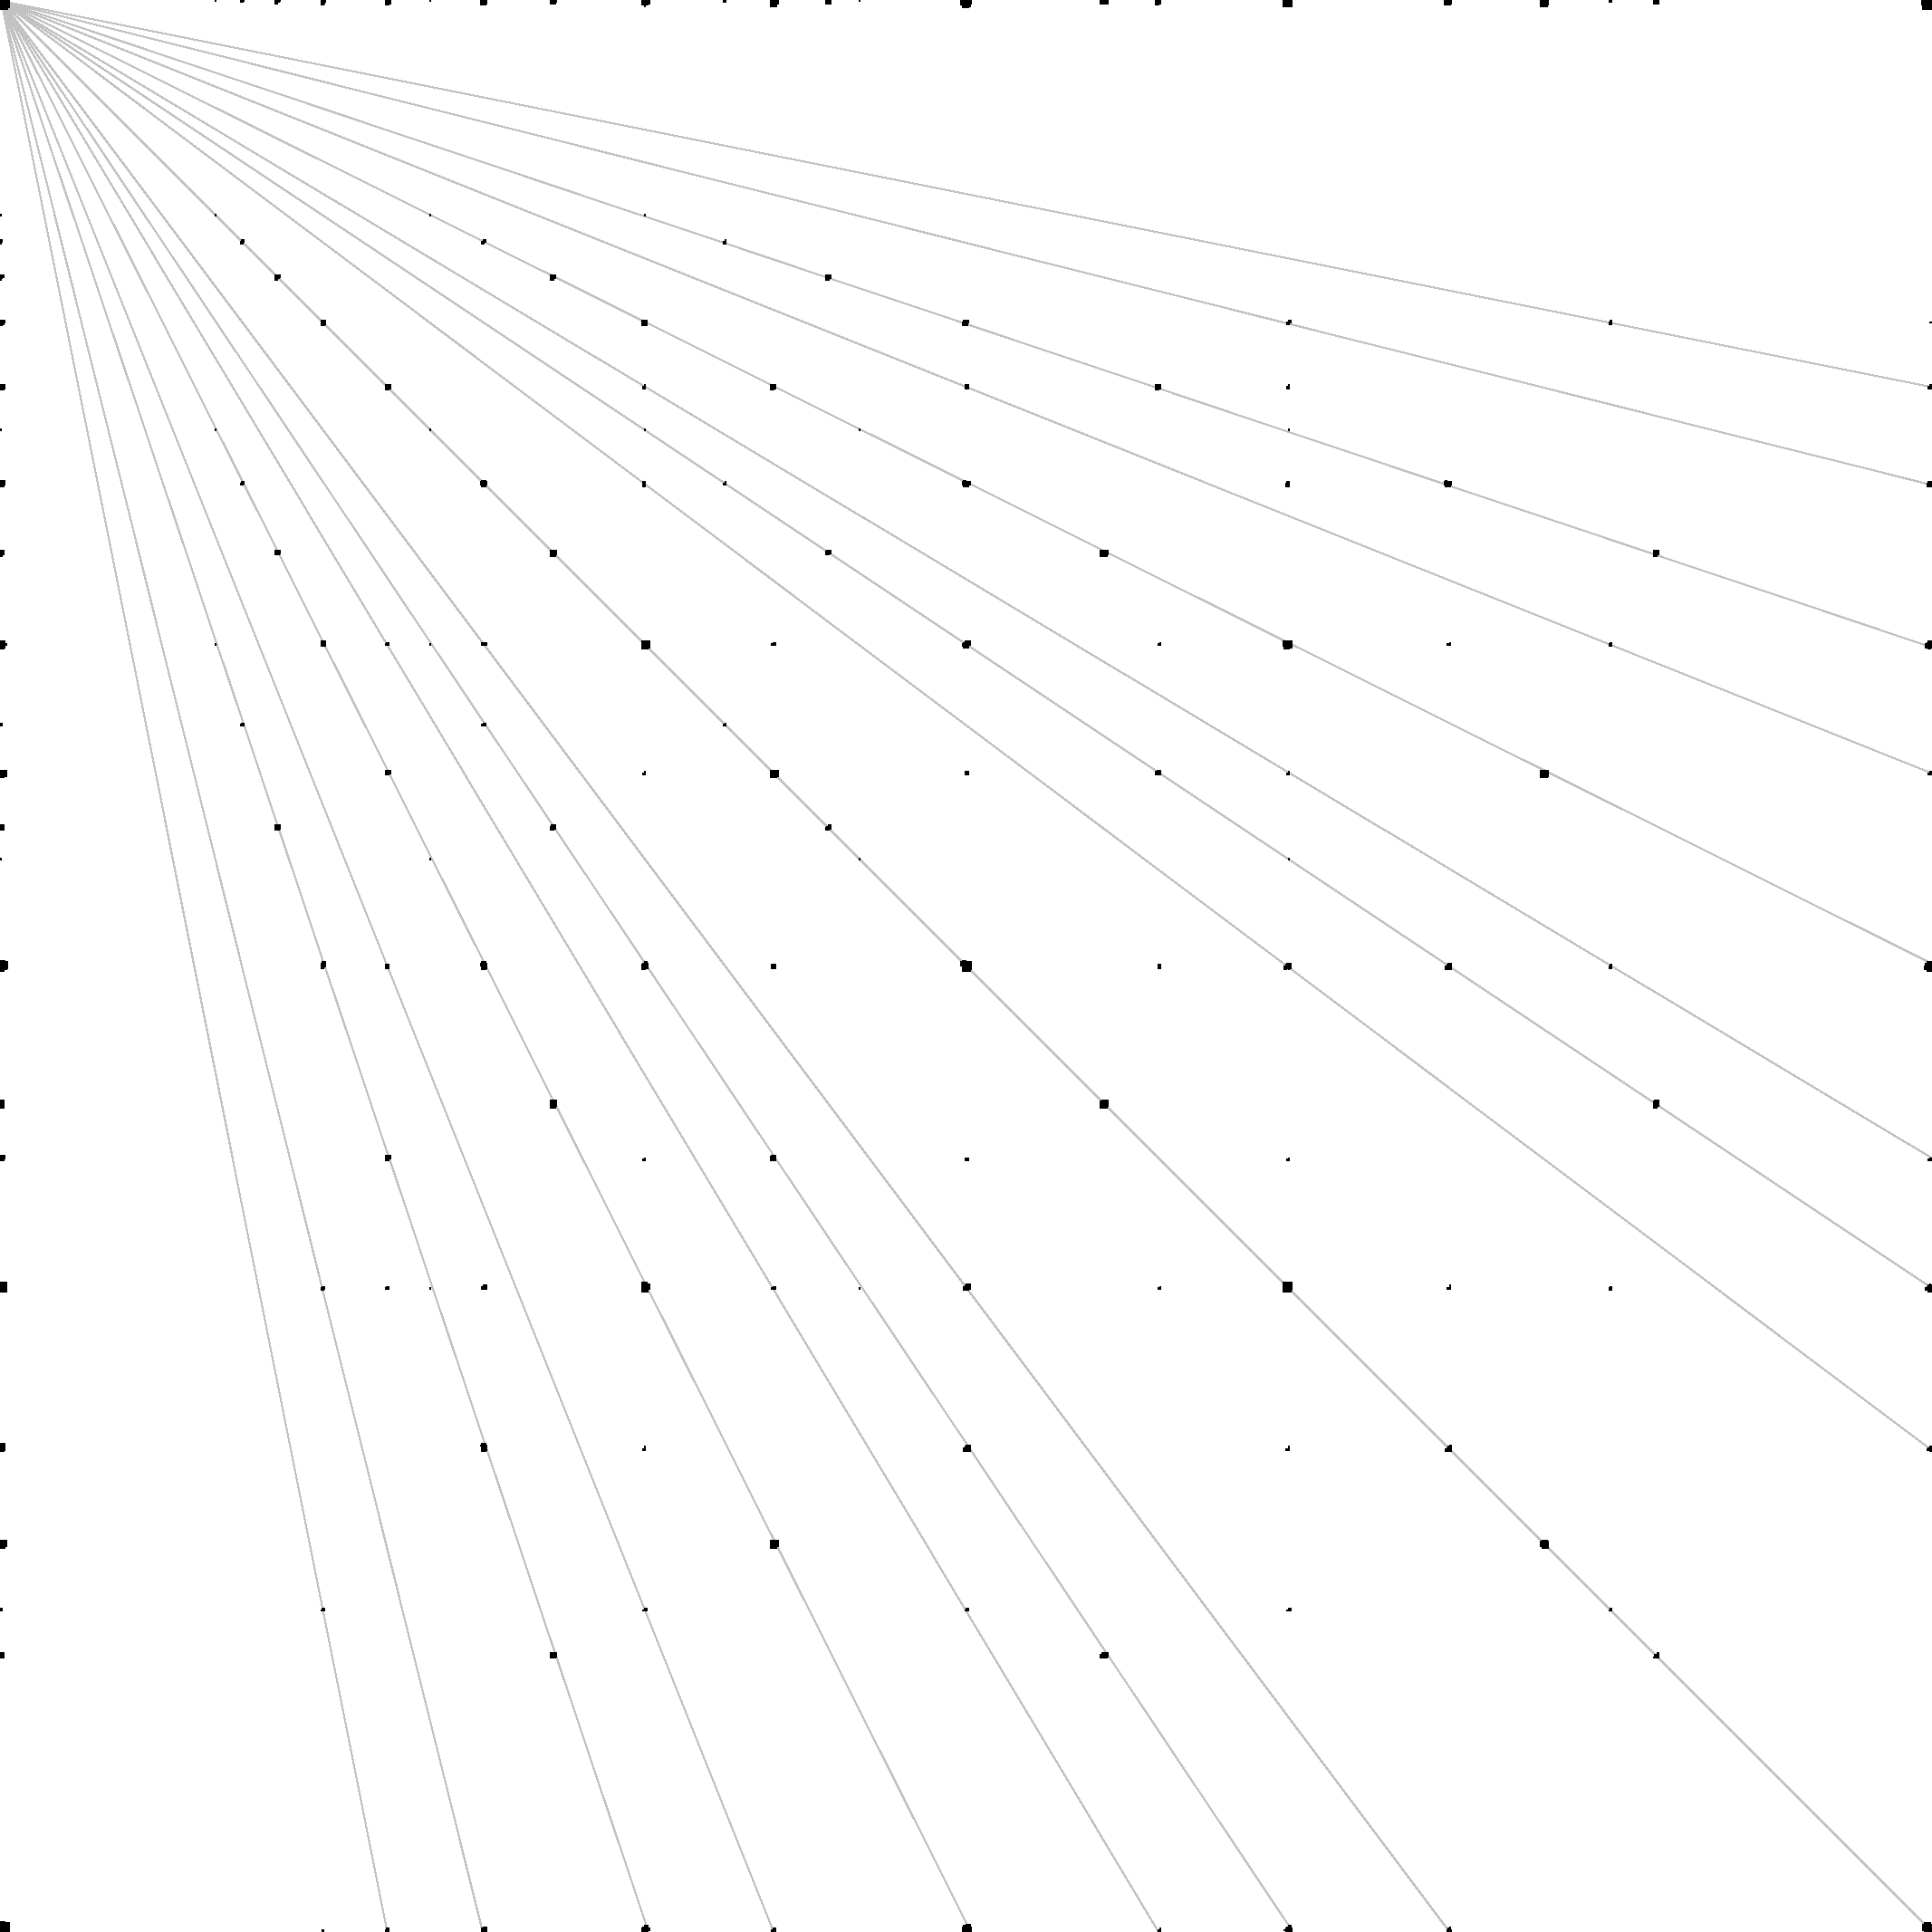
\includegraphics[width=0.90 \linewidth]{powerday3.pdf}
\end{center}\vspace{-0.1in}
\caption{All possible outcomes for the first two players in 3-player
  power days. These are the same games as the 3-player power hours,
  but at this scale makes it clear the groupings and their sparsity in
  the limit. Lines plotted from $\langle 0,0 \rangle$ to $\langle 60,
  k_2 \rangle$ and $\langle k_1, 60 \rangle$ show significant
  structure, but don't explain some of the interior points. These are
  probably games where a player participates in two cycles of
  different periods.
}
\label{fig:powerday3}
\end{figure}

The less extreme \kn\ Power-Three-Hours appears in
Figure~\ref{fig:powerthreehours}.

\begin{figure}
\begin{center}
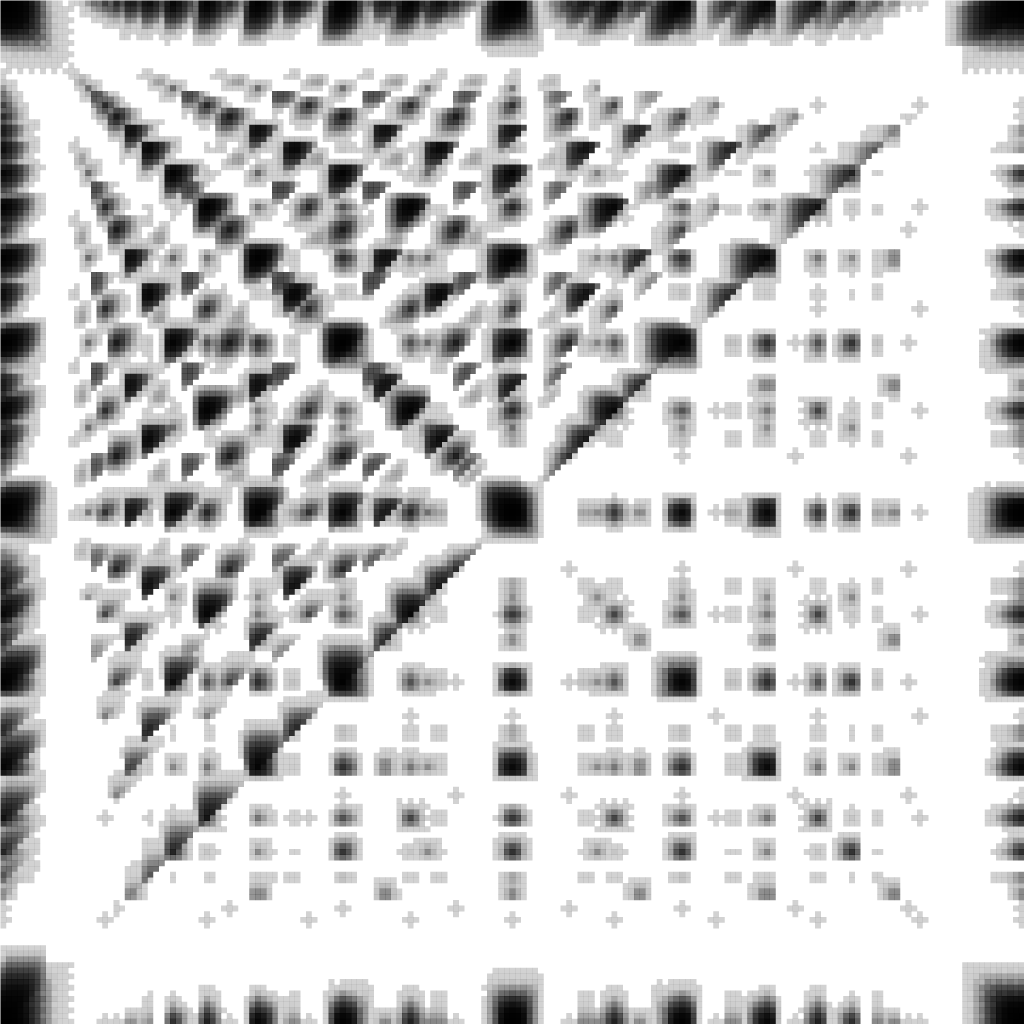
\includegraphics[width=0.90 \linewidth]{sample180min2players7states.png}
\end{center}\vspace{-0.1in}
\caption{6,456,764,116 samples of two-player BM7L Power Three-Hours.
}
\label{fig:powerthreehours}
\end{figure}


\section{Conclusion}

This section summarizes the known bounds for \bmsl, and states some
conjectures, before concluding.

\subsection{Known results}
\begin{enumerate}
  \item With one player, we have exact bounds on what is possible in
    the generalized case. With 8 cup states, a single player can
    drink 0--60 shots. Since each player can just play independently,
    this result extends to any number of players in BM8L. With fewer
    than 8 cup states, not every $k$ can be achieved alone.
  \item With two players in BM3L or BM4L, it is not possible for one
    of the players to drink every $k$ even if the other player helps her
    out.
  \item With two players, we know that BM5L does allow one player to
    drink any $k_1$ if the other player assists. In fact we can
    achieve any $\langle k_1, k_2 \rangle$ where $k_2 \in \{ 0, 1 \}$.
    No other $k_2$ can be used universally, though of course many
    other combinations are possible
    (Figure~\ref{fig:composite2player}). Many pairs $\langle k_1, k_2
    \rangle$ are known to be unattainable; this was established by
    exhaustively testing all possible configurations.
  \item Open: Can BM6L achieve all $\langle k_1, k_2 \rangle$? Seems
    unlikely, given that random exploration plateaus with about 95.65\%
    of the grid filled.
  \item BM7L can achieve all $\langle k_1, k_2 \rangle$. This was
    established by sampling random games until we found an example
    for every $\langle k_1, k_2 \rangle$.
  \item With three players in BM3L, one player can drink any number of
    shots if the other two players help.
\end{enumerate}

\subsection{Conjectures} \label{sec:conjectures}


\paragraph{Freedom: With two friends, you can drink any amount.} We know
that in a three-player game of BM3L, one of the three players can
drink the $k$ of her choice. This straightforwardly extends to $3
\times p$-player BM3L games. The {\bf Freedom} conjecture is that
with $p + 2$ players in BM3L, $p$ of them may have their choice of
$k_1 \ldots k_n$ drinks. If this conjecture fails, it probably fails
for 4 players, which might have a feasible enumeration strategy.

\paragraph{Teetotaller: Someone can drink nothing.} When $\langle k_1, 
\ldots, k_i, \ldots, k_p \rangle$ is achievable in \bmsl, so is
$\langle k_1, \ldots, 0, \ldots, k_p \rangle$. This conjecture would
be trivial if not for the rule that requires us to drink the contents
of a full cup if we want to pass it in a different state. This
conjecture is true for all the graphics presented in this
paper;\footnote{Actually, it is not established for (only) 11 minutes
  in Figure~\ref{fig:powerthreehours}, but this is not a proper
  \bmsl\ game as it takes place over 180 minutes. There should be
  solutions for 11, like in Figure~\ref{fig:dual11-53}; this is just
  a sample.} we can see that
cells in the 0 column are always filled when some other cell in that
row is filled. If this conjecture fails, it probably fails for BM1L or
BM2L which have the least freedom per player.

\medskip

In this paper I presented some new results in \kn\ Power-Hour theory, as
well as correct the historical record of some inebriated missteps. We
saw that stochastic simulation, abstract interpration, and sampling
are powerful tools for solving combinatorial drinking problems. We
established some firm results for the classic game and some bounds for
generalizations, as well as informally looked at some visualizations
of its geometric structure. However, there are still several open
problems in this field that demand further study.

\bibliography{paper}{}
\bibliographystyle{plain}
\end{document}
